\documentclass{article}
\usepackage[english]{babel}
\usepackage[letterpaper,top=2cm,bottom=2cm,left=3cm,right=3cm,marginparwidth=1.75cm]{geometry}

\usepackage{amsmath, amsfonts, amssymb}
\usepackage{amsthm}
\usepackage{graphicx}
\usepackage{algorithm}
\usepackage[noend]{algpseudocode}
\usepackage{xspace}
\usepackage{gensymb}
\usepackage{float}
\usepackage{appendix}
\usepackage{caption}
\captionsetup[table]{skip=3pt}
\usepackage{wrapfig}
\setlength{\columnsep}{1.5em}
\usepackage{comment}

\usepackage{xr-hyper}
\usepackage[colorlinks=true, allcolors=blue]{hyperref}
\usepackage[capitalize]{cleveref}

\crefname{figure}{fig.}{figs.}
\Crefname{figure}{Fig.}{Figs.}
\crefname{equation}{eq.}{eqs.}
\Crefname{equation}{Eq.}{Eqs.}
\crefformat{equation}{Eq.~#2#1#3}
\Crefformat{equation}{Eq.~#2#1#3}
\crefname{table}{table}{tables}
\Crefname{table}{Table}{Tables}
\crefname{algorithm}{alg.}{algs.}
\Crefname{algorithm}{Alg.}{Algs.}
\usepackage{authblk}

% 定理環境
\theoremstyle{plain}
\newtheorem{theorem}{Theorem}[section]
\newtheorem{lemma}[theorem]{Lemma}
\theoremstyle{definition}
\newtheorem{definition}[theorem]{Definition}
\theoremstyle{remark}
\newtheorem{remark}[theorem]{Remark}
\newtheorem{proposition}[theorem]{Proposition}

\renewcommand{\appendixpagename}{Supplemental Information}
\renewcommand{\appendixtocname}{Supplemental Information}

% カスタムコマンド（既存）
\input{commands}

% Reference
\usepackage{csquotes}
\usepackage[
    style=numeric-comp,
    backend=biber,
    sorting=none,
    date=year,natbib,
    maxnames=10,
    minnames=1,
    doi=true,
    url=true
]{biblatex}

\DeclareFieldFormat{labelnumberwidth}{#1.}
\DeclareFieldFormat{shorthandwidth}{#1.}
\setlength{\biblabelsep}{0.5em}

\addbibresource{citation_biophysj.bib}

\DeclareDelimFormat{finalnamedelim}{\addspace and\space}
\DeclareDelimFormat{multinamedelim}{\addcomma\space}

\AtEveryBibitem{
  \iffieldundef{doi}
    {}
    {\clearfield{url}}
}
\usepackage{fontspec}
\setmainfont{Helvetica}
\pagestyle{empty}

\externaldocument{biophysj}

\begin{document}

\setcounter{section}{0}
\renewcommand{\thesection}{S\arabic{section}}
\setcounter{equation}{0}
\renewcommand{\theequation}{S\arabic{equation}}
\setcounter{figure}{0}
\renewcommand{\thefigure}{S\arabic{figure}}
\setcounter{table}{0}
\renewcommand{\thetable}{S\arabic{table}}
\setcounter{algorithm}{0}
\renewcommand{\thealgorithm}{S\arabic{algorithm}}

\section{Navigating scheduling}
\label{sec:nav_scheduling}

We investigated how the navigating schedule $\eta_t$ in \Cref{eq:af3-guided} affects the navigating of \AFiii structure generation.
The conditional generation process in \AFiii is formulated as:

\begin{equation}
    \begin{split}
        X_{t_{i+1}} = X_{t_i} - \eta (t_{i+1} - \hat{t}_i) \bigl( \nabla_{X_{t_i}} \log p_{t_i}(X_{t_i} | a) - \eta_{t_i} \nabla_{X_{t_i}} \mathcal{L}_{\text{MSE}}(X_{t_i}) \bigr) + \lambda \bigl({\hat{t}_i^2 - t_i^2}\bigr)^{1/2} \epsilon,
        \label{eq:af3-guided-hatt}
    \end{split}
\end{equation}
where $i$ propagates from $1$ to $N$ and $\eta_t$ dominates the strength of the navigation.

Prior work commonly used simple schedules—--e.g., a constant value \cite{maddipatla2025inverse} or a mid-trajectory sigmoid \cite{raghu2025multiscale}—--
but, to our knowledge, there has not been a systematic quantification of how these choices affect generated structures.
Here, across different navigating schedules, we evaluated the trade-off
between the accuracy of following the target CV values and the physical plausibility of the generated structures,
and found an optimal navigating parameter set.

\paragraph{Navigating family and design of the sweep.}
We defined navigating schedules $\eta_t$ from the sigmoidal family defined in \Cref{eq:sigmoid}.
Specifically, we vary two hyperparameters that determine \emph{when} navigating turns on ($\tau_{\text{start}}$) and \emph{how strong} it becomes at the end ($y_{\text{max}}$).
For the two hyperparameters, we select five candidate values each:
$\tau_{\text{start}}$ is chosen at evenly spaced points in $[0.4,0.9]$,
and $y_{\text{max}}$ is chosen at evenly spaced points in $[0.6,1.6]$.
By evaluating all combinations of these choices, we obtained $5\times 5 = 25$ distinct schedule settings in total.
For each setting we generated five independent conformations and computed the averages of evaluation metrics of them.

\begin{equation}
    \begin{split}
        &\eta_{t_i} =
        \frac{y_{\text{max}}}{2}
        \frac{\| \delta \|_2}{\| g \|_2}
        \left(
            1 +
            \frac{\tanh\!\left( \alpha(\tau_i - \beta) / 2 \right)}
                 {\tanh\!\left( \alpha\beta / 2 \right)}
        \right),
        \\
        &\tau_i = \frac{i / N - \tau_{\text{start}}}{1 - \tau_{\text{start}}},
        \\[1.5ex]
        &\delta = \nabla_{X_{t_i}}\log p_{t_i}(X_{t_i}),
        \quad
        g = - \nabla_{X_{t_i}} \mathcal{L}_{\text{MSE}}(X_{t_i}),
        \\
        &\alpha = 10.0, \quad \beta = 0.5.
        \label{eq:sigmoid}
    \end{split}
\end{equation}

\paragraph{Systems and CVs}
Here, we describe the choice of protein system and the CVs on which restraints are applied.
The way restraints are imposed can in principle depend on factors such as protein size or the specific CVs chosen,
but our goal is to provide a concrete reference point that can serve as a guideline when users consider how to set the navigation strength.

In these experiments, we investigated the relationship between the navigation strength and the physical plausibility of the generated structures for both \AK (214 residues) and \flhac (346 residues).
The choice of CVs used for applying the navigation was, for \AK, LID–CORE, CORE–AMPbd, and AMPbd–LID, and for \flhac, \acdi–\acdiv and \acdii–\acdiii.
For \flhac, this schedule sweep deliberately used only these two CVs as a reduced subset to keep the parameter scan tractable; the final inference reported in the main text (and the full CV set listed in \Cref{tab:afm_settings}) additionally includes \acdii–\acdiv, for three CVs in total.
Because the guidance schedule controls the overall restraint strength rather than the specific CV set, we adopted the same schedule parameters ($\tau_{\text{start}}=0.6$, $y_{\text{max}}=0.6$) for the three-CV final inference.
As a reference, under navigation-free conditions, \AFiii predicts structures with inter-domain distances of $(2.85~\mathrm{nm},$ $2.19~\mathrm{nm},$ $3.45~\mathrm{nm})$ for \AK, and $(3.47~\mathrm{nm},$ $4.38~\mathrm{nm})$ for \flhac.
We conducted two types of experiments for these proteins:
(i) \textbf{in-distribution targets}, which correspond to physically plausible inter-domain distances observed in MD simulations. Specifically, $(2.41~\mathrm{nm},$ $2.01~\mathrm{nm},$$2.68~\mathrm{nm})$ was chosen for \AK and $(2.5~\mathrm{nm},$$4.5~\mathrm{nm})$ for \flhac.
(ii) \textbf{out-of-distribution targets}, which represent physically implausible inter-domain distances not observed in MD simulations. In this case, $(1.21~\mathrm{nm},$$1.51~\mathrm{nm},$$0.53~\mathrm{nm})$ was chosen for \AK and $(2.0~\mathrm{nm},$$3.0~\mathrm{nm})$ for \flhac.

\paragraph{Results}
A close examination of the MSE and MolProbity-score landscapes for each scheduling setting reveals that, for both the in-distribution and out-of-distribution targets, the two landscapes exhibit clearly distinct behaviors.
Notably, in the lower-left region of the parameter space, the relationship between the two metrics does not follow the simple rule that high MSE corresponds to low MolProbity-score (or vice versa).
Instead, when the navigation is initiated early (small $\tau_{\text{start}}$) and the maximum guidance strength is kept low (small $y_{\text{max}}$), both the MSE and the MolProbity-score tend to take low values.
This indicates the presence of a regime in which restraints can be applied without substantially degrading the geometric quality of the generated structures.
Based on these observations, in our study we adopt $\tau_{\text{start}}=0.6$ and $y_{\text{max}}=0.6$ that allow effective navigation without substantially degrading structural quality.
All evaluated schedules are shown in \Cref{fig:guidance_scheduling}, and the detailed results for \AK and \flhac are presented in \Cref{fig:guidance_scheduling_ak} and \Cref{fig:guidance_scheduling_flhac}, respectively.

\begin{figure}[H]
    \centering
    
\includegraphics[width=0.9\linewidth]{images/figure-7.pdf}
    \caption{
        All navigating schedulings evaluated in this study.
        The setting used in our main experiments, $\tau_{\text{start}}=0.6$ and $y_{\text{max}}=0.6$, is highlighted with a thick red line.
        }
    \label{fig:guidance_scheduling}
\end{figure}

\begin{figure}[htbp]
    \centering
    
\includegraphics[width=0.9\linewidth]{images/figure-8.pdf}
    \caption{
        \textbf{Results for \AK}. The upper 6 panels ((a)--(f)) shows results for the in-distribution target, and the lower 6 panels ((g)--(l)) shows results for the out-of-distribution target.
        \textbf{(a), (g)} Average MolProbity scores.
        \textbf{(b), (h)} Mean squared error (MSE).
        \textbf{(c), (i)} The inter-domain distance of estimated conformations (25 points, each one represents average inter-domain distance of corresponding schedule setting), with point colors representing the MolProbity scores.
        The cross point means that of the crystal structures (PDBID: 4AKE (open) and 1AKE (close)), and circle point means that of the target (every estimated structures were generated navigated towards this point).
        \textbf{(d), (e), (f), (j), (k), (l)} Evaluation metrics obtained during MolProbity scoring: clash score, Ramachandran favored rate (\%), and rotamer outlier rate (\%).
        }
    \label{fig:guidance_scheduling_ak}
\end{figure}

\begin{figure}[htbp]
    \centering
    
\includegraphics[width=0.9\linewidth]{images/figure-9.pdf}
    \caption{
        \textbf{Results for \flhac}. As before, the upper 6 panels ((a)--(f)) shows results for the in-distribution target, and the lower 6 panels ((g)--(l)) shows results for the out-of-distribution target.
        \textbf{(a), (g)} Average MolProbity scores.
        \textbf{(b), (h)} Mean squared error (MSE).
        \textbf{(c), (i)} The inter-domain distance of estimated conformations, with point colors representing the MolProbity scores.
        The cross point means that of the crystal structure (PDBID: 3A5I), and circle point means that of the target.
        \textbf{(d), (e), (f), (j), (k), (l)} Evaluation metrics obtained during MolProbity scoring: clash score, Ramachandran favored rate (\%), and rotamer outlier rate (\%).
        }
    \label{fig:guidance_scheduling_flhac}
\end{figure}

\section{Model implementation details}

\begin{algorithm}[H]
\caption{\textsc{Forward function of the $(\R^2, +) \rtimes C_8$-equivariant CNN}}
\label{alg:cnscnn}
\begin{algorithmic}
\State \textbf{Input:} $I \in \mathbb{R}^{B \times D \cdot N \times H \times W}$, $D=1$, $N=8$, $H=W=35$; \\
channels = [3,6,6,12,12,8], kernel\_size = [7,5,5,5,5,5], \\
$N_{\text{hidden-layers}} = 3$, $D_{\text{hidden}} = 64$, $D_{\text{out}} = N_{\text{domain-pairs}}$
\State \textbf{Output:} $\mathbf{D} \in \mathbb{R}^{B \times D_{\text{out}}}$

\State $I \gets \mathrm{R2Conv}(I;\, \text{in}=D \cdot N,\, \text{out}=\mathrm{channels}[0] \cdot N,\, k=\mathrm{kernel\_size}[0]) \to \mathrm{InnerBatchNorm} \to \mathrm{ReLU}$
\For{$i = 1 \to \mathrm{len(channels)}-1$}
    \State $I \gets \mathrm{R2Conv}(I;\, \text{in}=\mathrm{channels}[i-1]\!\cdot N,\, \text{out}=\mathrm{channels}[i]\!\cdot N,\, k=\mathrm{kernel\_size}[i])$
    \State $I \gets \mathrm{InnerBatchNorm}(I) \to \mathrm{ReLU}(I)$
    \If{$i \bmod 2 = 0$}
        \State $I \gets \mathrm{PointwiseAvgPoolAntialiased}\!\left(I;\sigma,\,s\right)$
        \State $\text{where}\quad
        \sigma=0.66, \quad
        s=
        \begin{cases}
        2 & \text{if size odd}\\
        1 & \text{if size even}
        \end{cases}$
    \EndIf
\EndFor

\State $I' \gets \mathrm{GroupPooling}(I)$ \hfill $I' \in \mathbb{R}^{B \times \mathrm{channels}[-1] \times H' \times W'}$
\State $I'' \gets \mathrm{PointwiseAvgPool}(I')$ \hfill $I'' \in \mathbb{R}^{B \times \mathrm{channels}[-1] \times 1 \times 1}$
\State $\mathbf{z} \gets \mathrm{Flatten}(I'')$ \hfill $\mathbf{z} \in \mathbb{R}^{B \times \mathrm{channels}[-1]}$
\State $\mathbf{h} \gets \mathrm{Linear}(\mathbf{z};\, \text{in}=\mathrm{channels}[-1],\, \text{out}=D_{\text{hidden}}) \to \mathrm{BatchNorm1d} \to \mathrm{ELU}$ \hfill $\mathbf{h} \in \mathbb{R}^{B \times D_{\text{hidden}}}$
\For{$j = 1 \to N_{\text{hidden-layers}}-1$}
    \State $\mathbf{h} \gets \mathrm{Linear}(\mathbf{h};\, \text{in}=D_{\text{hidden}},\, \text{out}=D_{\text{hidden}}) \to \mathrm{ReLU}(\mathbf{h})$ \hfill $\mathbf{h} \in \mathbb{R}^{B \times D_{\text{hidden}}}$
\EndFor
\State $\mathbf{D} \gets \mathrm{Linear}(\mathbf{h};\, \text{in}=D_{\text{hidden}},\, \text{out}=D_{\text{out}})$ \hfill $\mathbf{D} \in \mathbb{R}^{B \times D_{\text{out}}}$
\State \Return $\mathbf{D}$
\end{algorithmic}
\end{algorithm}

\begin{algorithm}[H]
\caption{\textsc{Forward function of the ResNet-18 embedding model}}
\label{alg:resnet}
\begin{algorithmic}
\State \textbf{Input:} $I \in \mathbb{R}^{B \times 1 \times H \times W}$, $H = W = 35$
\State \textbf{Output:} $\mathbf{z} \in \mathbb{R}^{B \times 256}$ on the unit hypersphere

\State \Comment{Backbone: ResNet-18 (ImageNet pretrained, conv1 modified for 1-channel input)}
\State $I \gets \mathrm{Conv2d}(I;\, \text{in}=1,\, \text{out}=64,\, k=7,\, s=2,\, p=3) \to \mathrm{BatchNorm2d} \to \mathrm{ReLU} \to \mathrm{MaxPool}$
\State $\mathbf{f} \gets \mathrm{ResNet\text{-}18\_layers}(I)$ \hfill $\mathbf{f} \in \mathbb{R}^{B \times 512 \times H' \times W'}$
\State $\mathbf{h} \gets \mathrm{GlobalAvgPool}(\mathbf{f})$ \hfill $\mathbf{h} \in \mathbb{R}^{B \times 512}$

\State \Comment{Projection Head}
\State $\mathbf{h} \gets \mathrm{Linear}(\mathbf{h};\, \text{in}=512,\, \text{out}=512) \to \mathrm{BatchNorm1d} \to \mathrm{ReLU}$
\State $\mathbf{h} \gets \mathrm{Linear}(\mathbf{h};\, \text{in}=512,\, \text{out}=256)$

\State \Comment{L2 normalization to unit hypersphere}
\State $\mathbf{z} \gets \mathbf{h} / \|\mathbf{h}\|_2$ \hfill $\mathbf{z} \in \mathbb{R}^{B \times 256}$, $\|\mathbf{z}\|_2 = 1$

\State \Return $\mathbf{z}$
\end{algorithmic}
\end{algorithm}

\section{Supplemental tables}

\begin{table}[H]
    \centering
    \caption{
        Key hyperparameters for the guided diffusion process used in this study.
        The guidance schedule parameters were selected on the basis of the systematic sweep described in \Cref{sec:nav_scheduling} (see also \Cref{fig:guidance_scheduling,fig:guidance_scheduling_ak,fig:guidance_scheduling_flhac}).
    }
    \label{tab:guidance_params}
    \begin{tabular}{lcl}
        \hline
        Parameter & Value & Description \\
        \hline
        \multicolumn{3}{l}{\textit{Guidance schedule (\Cref{eq:sigmoid})}} \\
        \hline
        $\tau_{\text{start}}$ & 0.6 & Restraint onset (fraction of $N$) \\
        $y_{\text{max}}$ & 0.6 & Maximum guidance strength \\
        $\alpha$ & 10.0 & Sigmoid steepness \\
        $\beta$ & 0.5 & Sigmoid midpoint \\
        \hline
        \multicolumn{3}{l}{\textit{Training data generation}} \\
        \hline
        CV grid range & $\pm 5.0$~nm around $\phi(X_{\text{ref}})$ & Range of target CV values \\
        CV grid step & 0.5~nm & Spacing of target CV grid \\
        \hline
    \end{tabular}
\end{table}

\begin{table}[hbt!]
    \centering
    \caption{MolProbity score thresholds used for geometric sanitization.}
    \label{tab:score_thresholds}
    \begin{tabular}{lc}
        \hline
        Criterion & Threshold \\
        \hline
        MolProbity Score & $\leq 4.0$ \\
        Clash Score & $\leq 70.0$ \\
        Ramachandran favored (\%) & $\geq 90.0$ \\
        Rotamer Outlier (\%) & $\leq 50.0$ \\
        \hline
    \end{tabular}
\end{table}

\begin{table}[H]
    \centering
    \caption{Settings for training pseudo-AFM images.}
    \label{tab:afm_settings}
    \begin{tabular}{lcc}
        \hline
         & \AK & \flhac \\
        \hline
        Lateral resolution [nm/pixel] & 0.3 & 0.98 \\
        Pixel size [pixel $\times$ pixel] & $35 \times 35$ & $35 \times 35$ \\
        Tip radius [nm] & $r \sim \mathrm{Uniform}(0.3,0.6)$ & $r \sim \mathrm{Uniform}(2.0,6.0)$ \\
        Tip apex angle [degree] & $a \sim \mathrm{Uniform}(10,30)$ & $a \sim \mathrm{Uniform}(10,30)$ \\
        Noise std. dev. [nm] & 0.0 & 0.5 \\
        Histogram matching & --- & \checkmark \\
        Dataset size [frames] & 5M & 5M \\
        Collective variables & Inter-domain distances & Inter-domain distances \\
                             & (LID-CORE, CORE-AMPbd, & (\acdi-\acdiv, \acdii-\acdiii, \\
                             & AMPbd-LID)  & \acdii-\acdiv)  \\
        \hline
    \end{tabular}
\end{table}

\section{Supplemental figures}

\begin{figure}[H]
    \centering
    
\includegraphics[width=0.8\linewidth]{images/figure-12.pdf}
    \caption{
        \textbf{Empirical rotation invariance of ResNet-18 embeddings}.
        For each molecular pose, simulated AFM images were generated at 8 in-plane rotation angles,
        and pairwise cosine similarity and geodesic distance in the embedding space were computed.
        Rotation pairs: cosine similarity $0.978 \pm 0.021$, geodesic distance $0.179 \pm 0.113$.
        Random (baseline) pairs: cosine similarity $0.924 \pm 0.049$, geodesic distance $0.374 \pm 0.125$.
        The substantially higher cosine similarity and lower geodesic distance for rotation pairs,
        well separated from the random baseline, confirm that the model has acquired
        empirical rotation invariance despite having no built-in rotational symmetry.
    }
    \label{fig:rotation_invariance}
\end{figure}

\begin{figure}[H]
    \centering
    
\includegraphics[width=\linewidth]{images/figure-10.pdf}
    \caption{
        \textbf{Selected candidate conformations for \AK and MolProbity evaluation for them}.
        \textbf{(a)} Projection of the candidate conformations into the inter-domain distance space.
        The following panels shows
        \textbf{(b)} MolProbity score,
        \textbf{(c)} Clash score,
        \textbf{(d)} Ramachandran favored rate (\%), and
        \textbf{(e)} Rotamer outlier rate (\%) of the candidate conformations.
        }
    \label{fig:ak_selection}
\end{figure}

\begin{figure}[H]
    \centering
    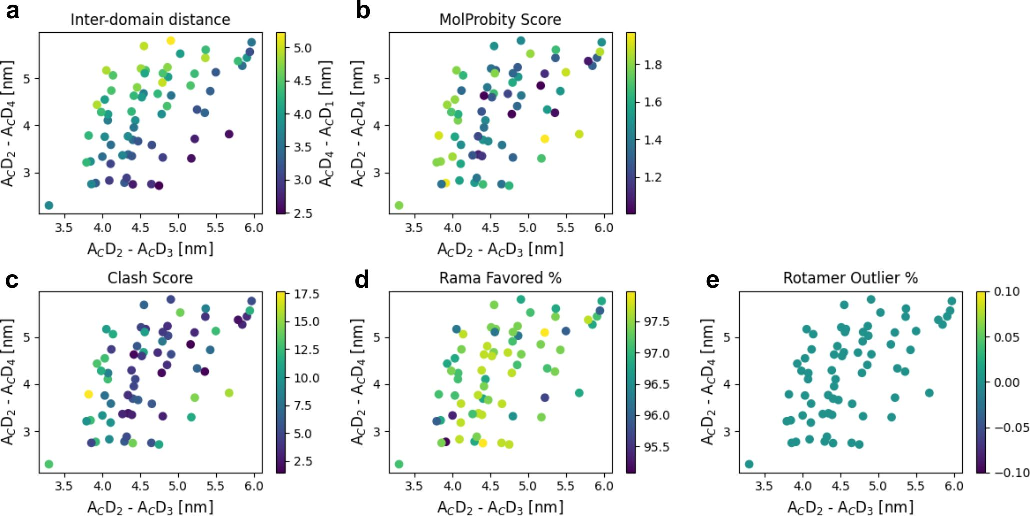
\includegraphics[width=1.0\linewidth]{images/figure-11.pdf}
    \caption{
        \textbf{Selected candidate conformations for \flhac and MolProbity evaluation for them}.
        \textbf{(a)} Projection of the candidate conformations into the inter-domain distance space.
        The following panels shows
        \textbf{(b)} MolProbity score,
        \textbf{(c)} Clash score,
        \textbf{(d)} Ramachandran favored rate (\%), and
        \textbf{(e)} Rotamer outlier rate (\%) of the candidate conformations.
        }
    \label{fig:flhac_selection}
\end{figure}


% supporting references
\printbibliography

\end{document}
